\documentclass[11pt]{article}
\usepackage[a4paper,margin=1in]{geometry}
\usepackage{amsmath,amssymb,amsthm,mathtools,booktabs,enumitem,graphicx,microtype}
\usepackage[colorlinks=true,linkcolor=blue,citecolor=blue]{hyperref}
\usepackage[nameinlink,capitalise]{cleveref}
\usepackage[numbers,sort&compress]{natbib}
\newtheorem{theorem}{Theorem}[section]
\newtheorem{corollary}[theorem]{Corollary}
\newtheorem{proposition}[theorem]{Proposition}
\theoremstyle{remark}\newtheorem{remark}[theorem]{Remark}
\newcommand{\norm}[1]{\left\lVert#1\right\rVert}
\title{Finite-Memory Three-Mode Capacity\\\large A Sharp Enclosure and Exterior-to-Fourth-Mode Recovery}
\author{Liang Wang}\date{July 2026}
\begin{document}\maketitle
\begin{abstract}
RH-109 showed that the normalized spectral four-volume factors as
$\nu_4=\Lambda_{23}q_4$, where
$q_4=s_4/s_1$ and
$\Lambda_{23}=(s_2/s_1)(s_3/s_1)$.  This paper isolates and controls the
capacity factor.  If $\widehat s_j$ are the singular values of a recent
projected cross and the forgotten-memory operator radius is $\delta$, we
prove
\[
 \frac{(\widehat s_2-\delta)_+(\widehat s_3-\delta)_+}
      {(\widehat s_1+\delta)^2}
 \le\Lambda_{23}\le
 \frac{(\widehat s_2+\delta)(\widehat s_3+\delta)}
      {(\widehat s_1-\delta)_+^2}.
\]
Dividing the RH-109 spectral-volume lower bound by the upper endpoint gives
a rigorous capacity-aware fourth-mode certificate.  On 360 archived
threshold-update records its support count agrees exactly with the direct
Weyl certificate: 113, 109, and 98 records at cutoffs
$10^{-8},10^{-6},10^{-4}$.  All 78 fine updates pass each cutoff, the minimum
fine recovery efficiency is $0.9982343$, and the widest fine capacity
interval is $0.1761\%$ of the true capacity.  At fixed normalized volume
$\nu$, capacity obeys the sharp universal interval
$\nu^{2/3}\le\Lambda_{23}\le1$.  Thus the factorization is now rigorous and
numerically lossless on the archived chain, but an independent physical
all-level capacity upper law remains open.  No Stage A, Hilbert--Polya,
zero-identification, or Riemann Hypothesis result is claimed.
\end{abstract}

\section{Introduction}
The source-seeded quotient route keeps four projected-cross directions when
$q_4=s_4/s_1$ exceeds an adaptive threshold
\citep{WangWeakMode2026,WangSupportLaw2026}.  RH-108 gave a recent-memory
Weyl certificate for this ratio, while RH-109 replaced the fourth mode by the
coordinate-free spectral four-volume
\citep{WangFourthCross2026,WangExterior2026}.  The replacement loses the
factor
\begin{equation}
 \Lambda_{23}(K)=\frac{s_2(K)s_3(K)}{s_1(K)^2},
 \qquad \nu_4(K)=\Lambda_{23}(K)q_4(K).
 \label{eq:factor}
\end{equation}
The purpose of this paper is to determine whether that factor can be paid
rigorously through the same finite-memory radius.

There are two questions.  First, how stable is $\Lambda_{23}$ under a small
operator perturbation?  Second, does dividing a volume lower bound by a
capacity upper bound recover enough of the direct fourth-mode certificate to
be useful?  Both have exact finite-dimensional answers.  The finite replay
then shows that the composition loses less than two parts in a thousand on
the fine scales.

\section{Capacity and finite-memory perturbations}
Let $K$ and $\widehat K$ map an $r$-dimensional packet into its complement,
and assume
\begin{equation}
 \norm{K-\widehat K}_2\le\delta.
 \label{eq:radius}
\end{equation}
Write $s_1\ge\cdots\ge s_r$ and
$\widehat s_1\ge\cdots\ge\widehat s_r$ for their singular values.  Set
\begin{equation}
 \ell_j=(\widehat s_j-\delta)_+,
 \qquad u_j=\widehat s_j+\delta.
 \label{eq:endpoints}
\end{equation}

\begin{theorem}[Finite-memory three-mode capacity enclosure]
\label{thm:capacity}
If $s_1>0$, then
\begin{equation}
 L_{23}^-:=\frac{\ell_2\ell_3}{u_1^2}
 \le \Lambda_{23}(K)
 \le L_{23}^+:=\frac{u_2u_3}{\ell_1^2},
 \label{eq:capacity-interval}
\end{equation}
where the upper endpoint is $+\infty$ when $\ell_1=0$.
\end{theorem}
\begin{proof}
Weyl's singular-value perturbation inequality gives
$\ell_j\le s_j\le u_j$ for every $j$
\citep{Bhatia1997,StewartSun1990}.  Insert the lower numerator and upper
denominator bounds for the left inequality, and the upper numerator and
lower denominator bounds for the right inequality.
\end{proof}

For normalized memory Gramians, RH-108 supplies
\[
 \delta_{t,m}=\eta^m\frac{1-\eta^{t-m+1}}{1-\eta}
\]
for a depth-$m$ recent cross.  Hence \cref{thm:capacity} is a directly
computable finite-memory enclosure.

\section{Capacity-aware volume recovery}
RH-109 proves the spectral-volume lower bound
\begin{equation}
 B_4^{\rm vol}=\frac{\ell_1\ell_2\ell_3\ell_4}{u_1^4}
 \le\nu_4(K).
 \label{eq:volume}
\end{equation}

\begin{theorem}[Exterior-to-fourth-mode recovery]
\label{thm:recovery}
Under the assumptions of \cref{thm:capacity},
\begin{equation}
 q_4(K)\ge B_4^{\rm cap}:=
 \begin{cases}
 B_4^{\rm vol}/L_{23}^+,&0<L_{23}^+<\infty,\\
 0,&\text{otherwise}.
 \end{cases}
 \label{eq:recovery}
\end{equation}
Moreover,
\begin{equation}
 B_4^{\rm cap}
 =\frac{\ell_4}{u_1}
 \left(\frac{\ell_1}{u_1}\right)^3
 \frac{\ell_2}{u_2}\frac{\ell_3}{u_3}
 \le\frac{\ell_4}{u_1}.
 \label{eq:efficiency}
\end{equation}
\end{theorem}
\begin{proof}
The exact identity \eqref{eq:factor} and
$\Lambda_{23}(K)\le L_{23}^+$ give
$q_4=\nu_4/\Lambda_{23}\ge B_4^{\rm vol}/L_{23}^+$.  Substitution of
\eqref{eq:volume} and \eqref{eq:capacity-interval} gives
\eqref{eq:efficiency}.  Every displayed efficiency factor is at most one.
\end{proof}

The theorem explains both the strength and the limitation of the
factorization.  When $\delta/\widehat s_j$ is small, the extra factors are
close to one and the direct Weyl ratio is recovered.  If an intermediate
singular value approaches the perturbation radius, the volume route loses
that direction before the direct fourth-mode numerator necessarily does.

\section{Sharp capacity range at fixed volume}
\begin{proposition}[Sharp fixed-volume capacity interval]
\label{prop:sharp}
For $0\le\nu_4\le1$,
\begin{equation}
 \nu_4^{2/3}\le\Lambda_{23}\le1,
 \label{eq:sharp}
\end{equation}
and both endpoints are attained.
\end{proposition}
\begin{proof}
RH-109 gives $\nu_4\le q_4\le\nu_4^{1/3}$.  Since
$\Lambda_{23}=\nu_4/q_4$, inversion yields \eqref{eq:sharp}.  The spectrum
$(1,1,1,\nu_4)$ gives $\Lambda_{23}=1$, while
$(1,\nu_4^{1/3},\nu_4^{1/3},\nu_4^{1/3})$ gives
$\Lambda_{23}=\nu_4^{2/3}$.
\end{proof}

The same endpoint spectra admit the trace-one source-seeded realization of
RH-109 with fixed memory clock and diagonal blocks.  Therefore no generic
normalized-memory argument can replace the upper endpoint one by a smaller
universal constant.

\section{Sharpness and reduced realization}
\label{sec:sharpness}

The capacity enclosure is sharp as a radius-only statement.  Fix numbers
$a>b>c>\delta$ and consider a recent diagonal cross whose first three
singular values are $a,b,c$, together with an admissible fourth value.  A
perturbation acting negatively on the second and third right singular
directions changes their values to $b-\delta$ and $c-\delta$, while a
perturbation acting positively on the first direction changes the leading
value to $a+\delta$.  Thus the lower endpoint in
\eqref{eq:capacity-interval} is attained in the diagonal model.  Reversing
the signs gives the upper endpoint.  No improvement can follow from the
single number $\norm{K-\widehat K}_2$ without additional alignment data.

The reduced-moment representation makes the same point intrinsically.  If
$C=K^*K$ has eigenvalues $\lambda_j=s_j^2$, then
\begin{equation}
 \Lambda_{23}(K)=\frac{\sqrt{\lambda_2\lambda_3}}{\lambda_1},
 \qquad
 q_4(K)=\frac{\sqrt{\lambda_4}}{\sqrt{\lambda_1}}.
 \label{eq:capacity-moment}
\end{equation}
For the recent memory, $C=M_2-A^2$ is a packet-sized matrix.  Hence the
capacity interval can be evaluated without an ambient complement solve, but
it still requires the second and third eigenvalues of that reduced matrix.
The moment reduction changes the representation of the calculation; it does
not create a lower bound on $\lambda_2$ or $\lambda_3$.

\begin{proposition}[Conditional capacity route]
\label{prop:conditional}
Suppose a physical family admits, for all sufficiently fine levels, a
volume lower bound $\nu_4\ge v_t>0$ and an independent capacity upper law
$\Lambda_{23}\le L_t$.  Then
\begin{equation}
 q_4\ge v_t/L_t.
 \label{eq:conditional}
\end{equation}
In particular, $v_t\ge\tau L_t$ implies the no-quotient support gate
$q_4\ge\tau$.
\end{proposition}
\begin{proof}
Divide the identity $\nu_4=\Lambda_{23}q_4$ by the positive upper bound
$L_t$.
\end{proof}

This proposition is deliberately conditional.  It identifies the exact
missing input for an all-level capacity route: one must obtain $v_t$ and
$L_t$ from independent physical estimates, rather than read both from the
same finite recent SVD.

\section{Five-scale audit}
We replay the two source-seeded channels at
$\sigma\in\{0.16,0.08,0.04,0.02,0.01\}$, the three thresholds
$10^{-8},10^{-6},10^{-4}$, memory ratio $\eta=1/512$, and recent depth five.
At each update the full cross is used only as a finite comparator.  The
certificate itself uses the recent spectrum and the guarded RH-108 tail.

\begin{table}[t]
\centering\small
\caption{Capacity-aware recovery counts versus direct Weyl counts.}
\begin{tabular}{@{}lrrr@{}}\toprule
cutoff & recovered & direct Weyl & fine recovered\\\midrule
$10^{-8}$ & $113/120$ & $113/120$ & $78/78$\\
$10^{-6}$ & $109/120$ & $109/120$ & $78/78$\\
$10^{-4}$ & $98/120$ & $98/120$ & $78/78$\\\bottomrule
\end{tabular}
\end{table}

\begin{table}[t]
\centering\small
\caption{Observed capacity ranges for the primary threshold chain.}
\begin{tabular}{@{}lrrr@{}}\toprule
scale & minimum $\Lambda_{23}$ & maximum $\Lambda_{23}$ & updates\\\midrule
$0.16$ & $1.07\times10^{-11}$ & $1.85\times10^{-3}$ & $8$\\
$0.08$ & $3.53\times10^{-6}$ & $1.87\times10^{-2}$ & $12$\\
$0.04$ & $1.72\times10^{-6}$ & $2.90\times10^{-1}$ & $22$\\
$0.02$ & $5.23\times10^{-5}$ & $3.44\times10^{-1}$ & $34$\\
$0.01$ & $1.39\times10^{-4}$ & $3.88\times10^{-1}$ & $44$\\\bottomrule
\end{tabular}
\end{table}

All 360 capacity intervals contain the actual factor and every recovery
implication is valid.  On the fine scales
\begin{align*}
 5.23356\times10^{-5}&\le\Lambda_{23}\le0.387636,\\
 \max\frac{L_{23}^+-L_{23}^-}{\Lambda_{23}}&=1.76065\times10^{-3},\\
 \min\frac{B_4^{\rm cap}}{\ell_4/u_1}&=0.9982343.
\end{align*}
Thus the volume/capacity decomposition reproduces the direct support gate to
better than $0.18\%$ on every fine record.  The maximum relative enclosure
width over all five scales is $0.0928$ and occurs in a weak coarse branch.

\begin{figure}[t]
\centering
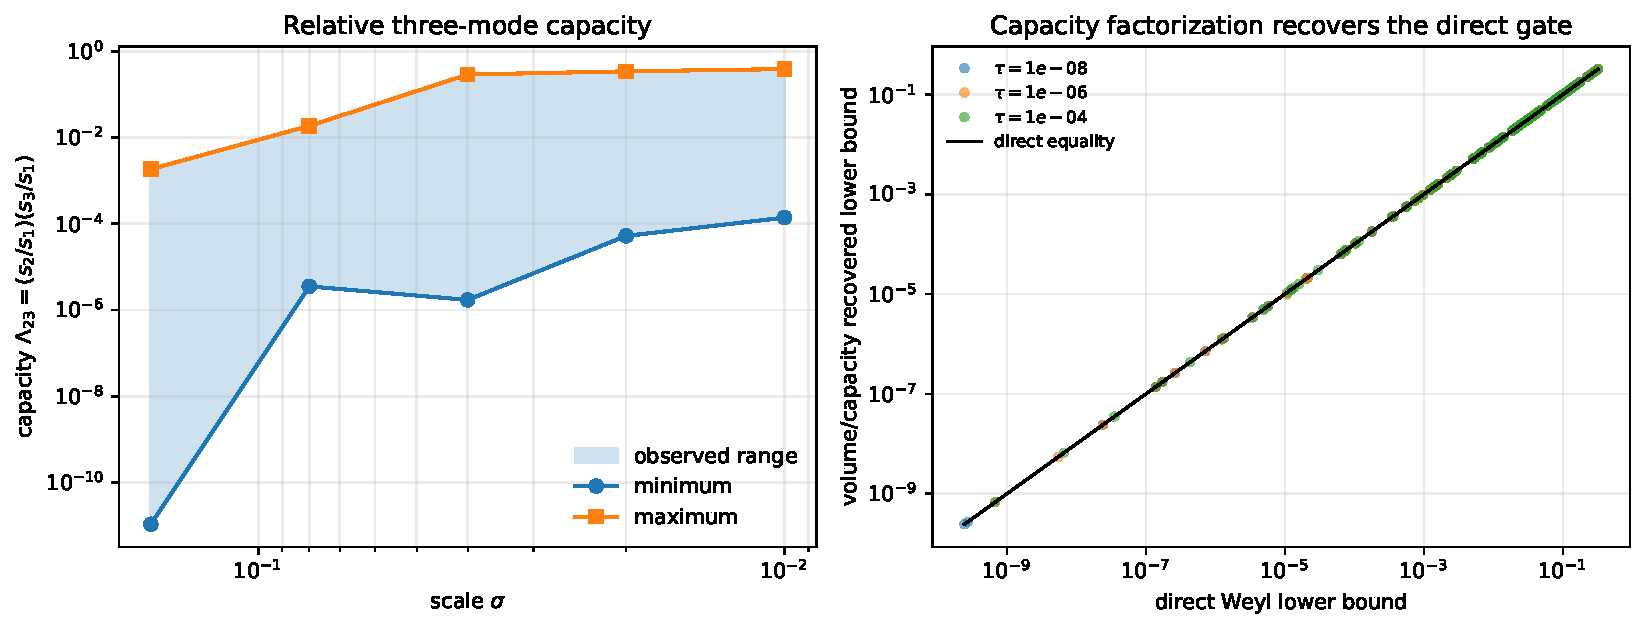
\includegraphics[width=\textwidth]{figures/finite_memory_three_mode_capacity.pdf}
\caption{Left: the physical capacity range across scales.  Right: the
capacity-aware recovery lower bound lies almost on the direct Weyl lower
bound; the remaining loss is exactly the product in \eqref{eq:efficiency}.}
\end{figure}

\section{Route consequence and claim boundary}
RH-110 closes the algebraic composition
\[
 \text{recent volume lower bound}+\text{recent capacity upper bound}
 \Longrightarrow\text{fourth-mode support}.
\]
It does not yet produce independent physical inputs: both factors are
currently extracted from the same recent singular spectrum.  An all-level
argument must replace at least the capacity upper endpoint by a simpler
source/observation, energy, or recurrence estimate, and must still prove a
physical volume lower bound.

The exact claims are the capacity enclosure, recovery theorem, sharp
fixed-volume interval, and finite five-scale validation.  Open are an
all-level capacity law, all-level exterior lower bound, unconditional
fine-support separation, and Stage A.  No Hilbert--Polya operator, zero
identification, prime-power trace formula, or Riemann Hypothesis conclusion
is asserted.

\section{Reproducibility}
\begin{verbatim}
PYTHONDONTWRITEBYTECODE=1 /root/math/.venv/bin/python \
  experiments/build_capacity_audit.py
PYTHONDONTWRITEBYTECODE=1 /root/math/.venv/bin/python \
  experiments/build_capacity_audit.py --smoke
MPLBACKEND=Agg PYTHONDONTWRITEBYTECODE=1 /root/math/.venv/bin/python \
  experiments/make_figures.py
PYTHONDONTWRITEBYTECODE=1 /root/math/.venv/bin/pytest -q -p no:cacheprovider
latexmk -pdf -interaction=nonstopmode -halt-on-error main.tex
cp main.pdf finite-memory-three-mode-capacity.pdf
\end{verbatim}
\bibliographystyle{plainnat}\bibliography{references}
\end{document}
